\section{Introduction} \label{sec:introduction}
% Vision
\showthe\font
\IEEEPARstart{T}{here} is a growing interest in deploying autonomous systems in unstructured environments to perform complex manipulation tasks for different applications like assistive service in the healthcare domain~\cite{cooper2020ari}, agrifoods~\cite{duckett2018agricultural}, and industrial inspection and maintenance~\cite{lattanzi2017review}. In those scenarios, the community is particularly interested in the manipulation of movable and articulated objects (like the furniture in \fig\ref{fig:royal_panda}) which poses additional challenges beyond those experienced in a static environment. Mobile manipulator robots present a compelling choice to tackle these problems since they combine an unconstrained workspace with highly dexterous interaction capabilities. However, to fully exploit these capabilities, systems require planning and control algorithms that can generate fast, accurate, and coordinated reactive whole-body motions that account for multiple potential contacts with the environment. 

\subsection{Related Works}

% Existing methods
While traditional ``plan-and-act'' frameworks break down manipulation tasks into subproblems that are easier to solve (e.g., reach, grasp, pull)~\cite{Murali2020}, they do not offer fast replanning, which is crucial for mobile manipulation in dynamic and uncertain environments.

With the recent advancements in artificial intelligence, reinforcement learning (RL) is a promising method to solve a range of robotic control tasks, including manipulation~\cite{finn2016deep}, as they learn an end-to-end representation of the optimal policy. However, real-world applications of RL typically require training times that are not practical for physical hardware and suffer from the well-known \textit{sim-to-real} gap~\cite{chebotar2019closing}. 
On the other side of the spectrum, Model Predictive Control (MPC) has gained broad interest in the robotics community thanks to its ability to deal with input constraints and task objectives by solving a multivariate optimization problem or using the \textit{principle of optimality}. 
MPC has been successfully applied to aerial robots~\cite{peric2021direct}, autonomous racing~\cite{liniger2015optimization}, legged locomotion~\cite{grandia2019frequency}, and whole-body control~\cite{minniti2019whole}. 
Nevertheless, MPC requires a model that is locally differentiable with respect to the input and the state~\cite{buchli2017optimal}. On the other hand, manipulation tasks involve changes in the contact state causing sharp discontinuities in both the cost and system dynamics, thus directly violating the differentiability requirements. 


\begin{figure}[t]
\centering
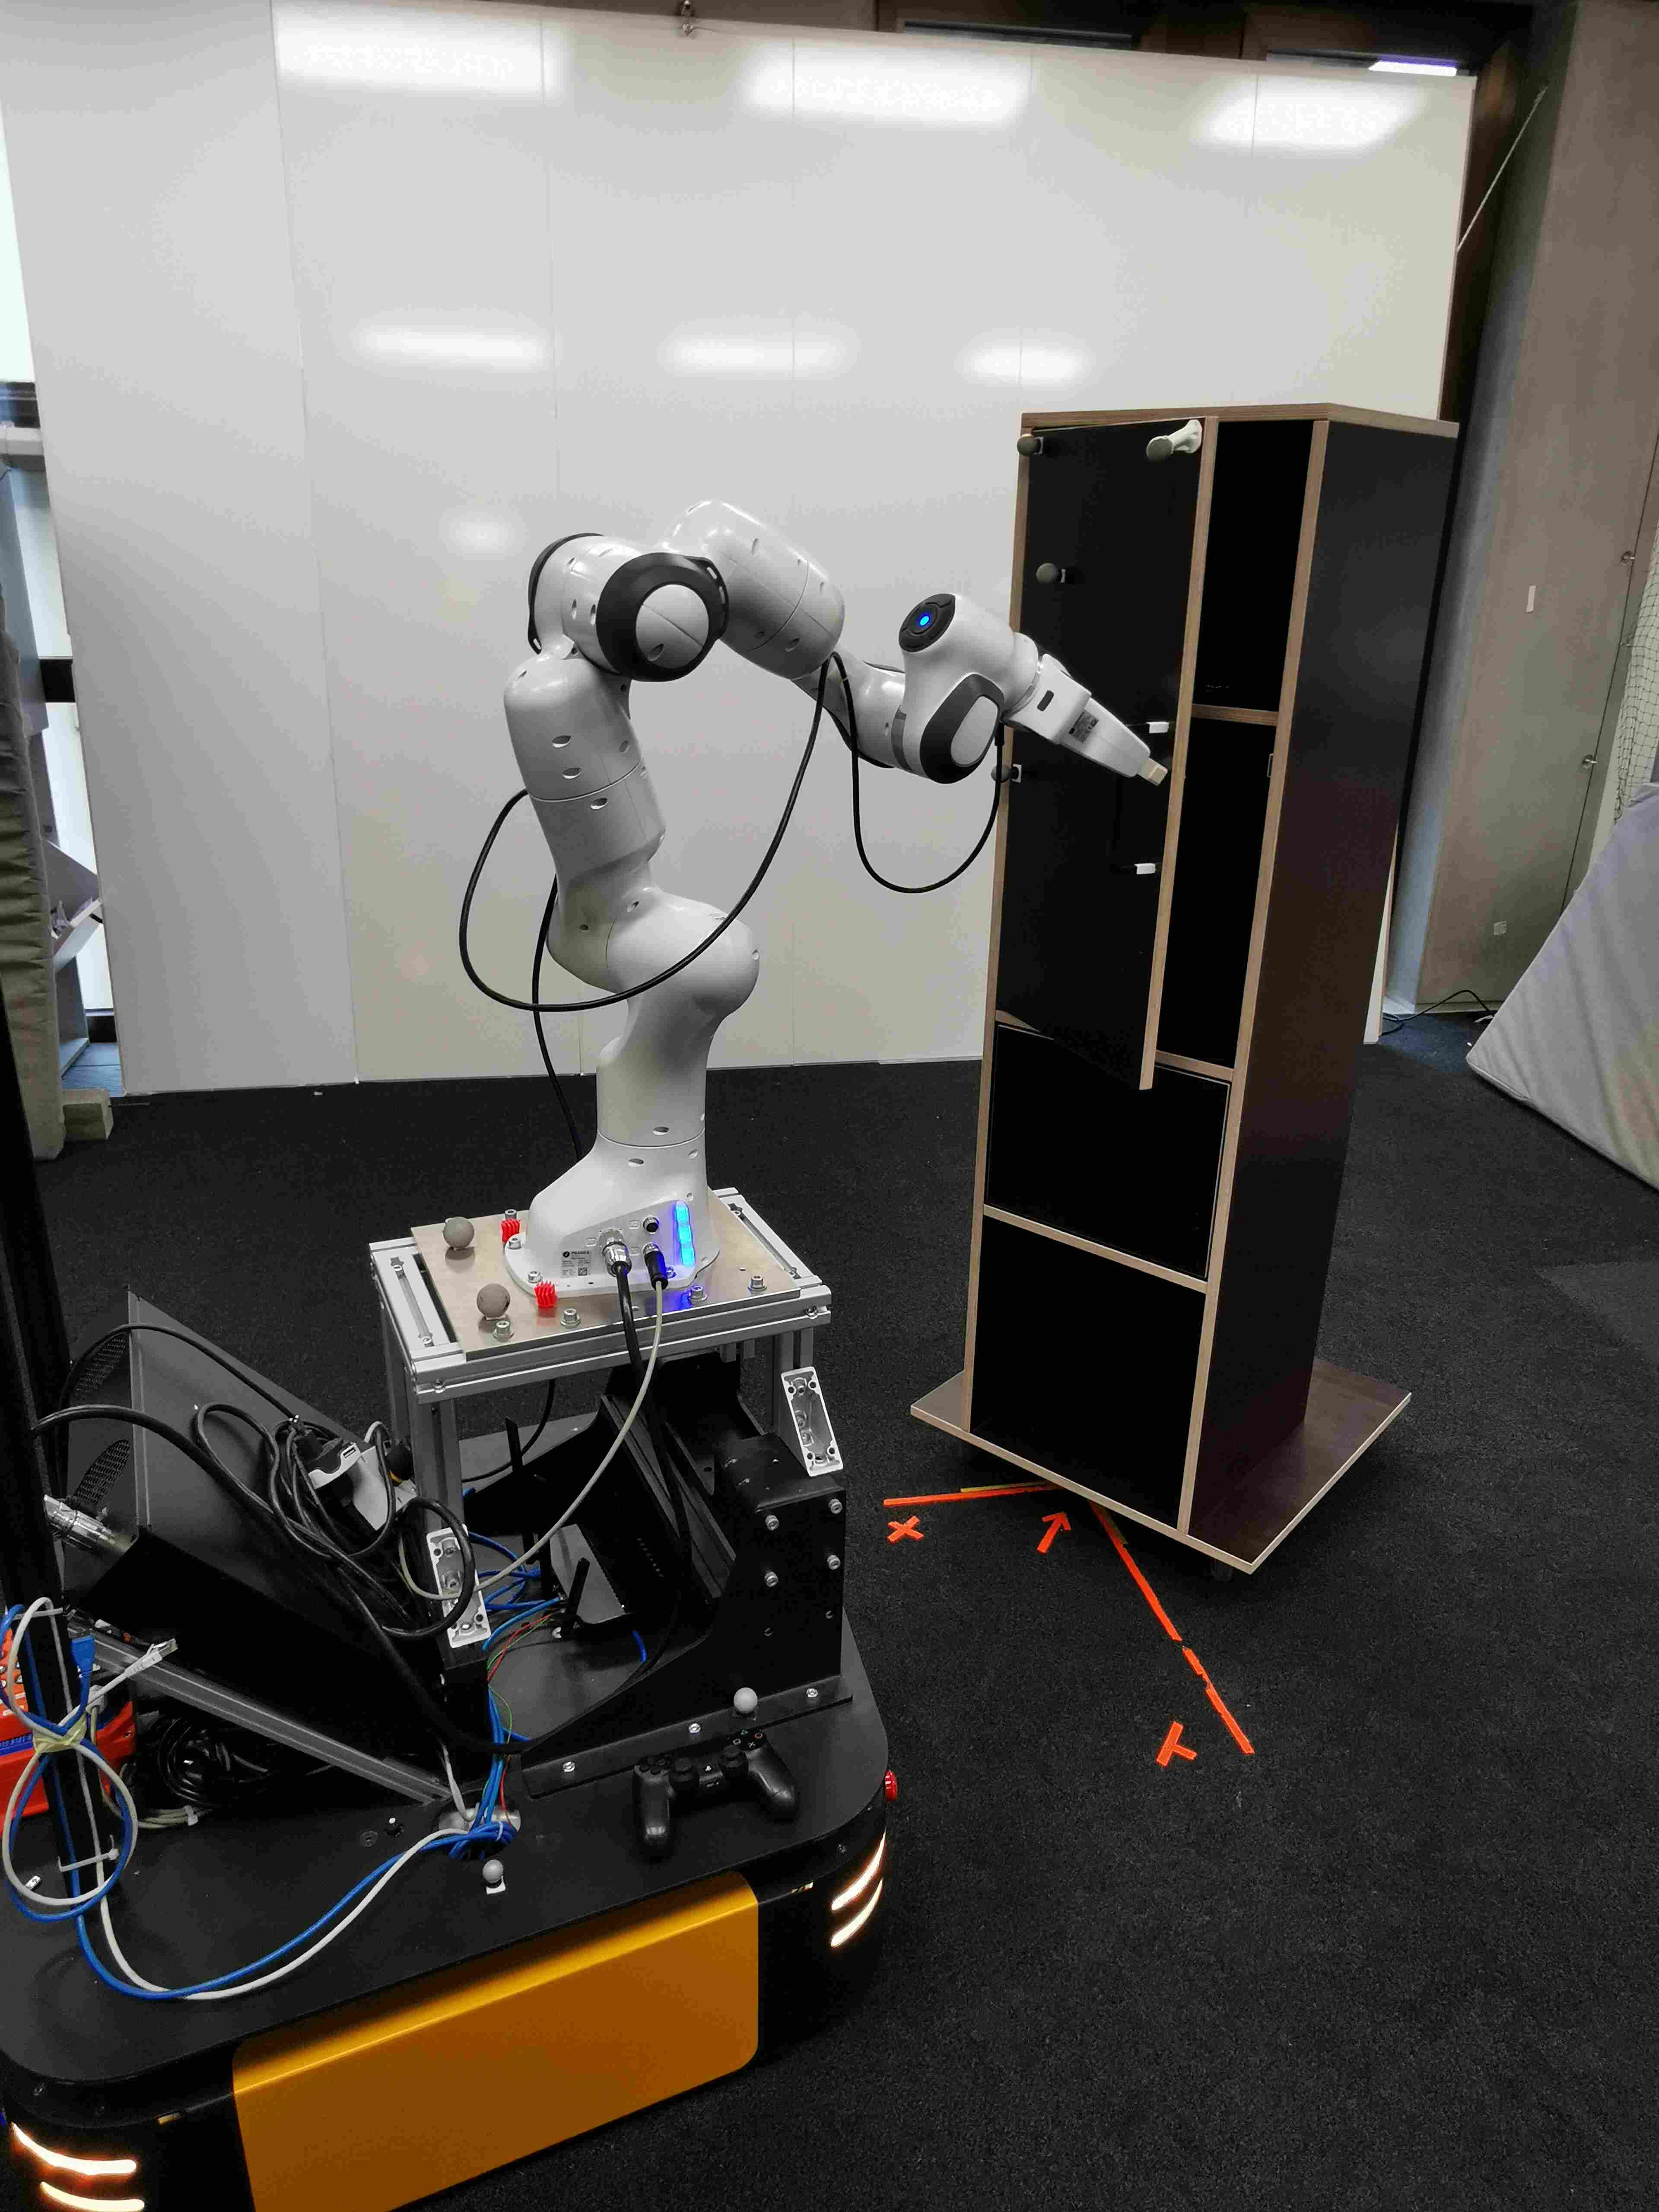
\includegraphics[trim={0 500 0 800},clip,width=0.8\columnwidth]{framework_manipulation/figures/hardware/system_figure_new.jpg}
\caption{\textit{RoyalPanda} (a 10-DOF mobile manipulator) while performing a door opening task.} \label{fig:royal_panda}
\end{figure}

% Performance : sampling control
Recently, sampling-based methods have emerged and advanced in theory and applications~\cite{lee_aggressive_2020,abraham_model-based_2020,williams_information_nodate,williams_information_2017,rajamaki_augmenting_2017}. 
In contrast to traditional MPC, sampling methods stem from a probabilistic interpretation of the control problem. 
Rather than solving a complex optimization problem, they rely on sampling system trajectories, referred to as \textit{rollouts}, and ``weighting'' them according to the cumulative cost so that only favorable trajectories survive the iterative sampling process. The only requirement is that it is possible to forward simulate the system evolution. This has been exploited to control camera motions for target tracking in drone racing~\cite{lee_aggressive_2020}, robot arm motions for manipulation tasks~\cite{abraham_model-based_2020}, and for generating aggressive driving maneuvers such as drifting~\cite{williams_information_nodate, williams_information_2017}. 

% Gap 
Demonstrations on real systems involving different physical interactions (e.g., a robot arm opening a drawer~\cite{abraham_model-based_2020}) have typically only been shown by breaking down the multi-contact task into stages and enforcing constraints when switching between them. \add{In this context, MPC is often used to track an externally provided reference trajectory. In \cite{minniti2019whole} for example, a circular trajectory is computed for a door opening task and the gripper is rigidly connected to the handle \emph{prior} to the interaction.}
This can limit the control envelope of the system and sacrifices solution optimality. For example, it is common practice to fix the gripper orientation between successive reach and pull stages and perform manipulation under a rigid grasp. In the presence of uncertainty and tracking errors, this often leads to high contact forces and dangerous behaviors.

\add{In particular, the opening task requires a big motion range that has to cope with the limited robot workspace induced by its joint limits. It is important to notice that the sampling based-controller is deployed as an interaction-aware and closed-loop reference generator. That means that if the gripper loses contact or the robot reaches its limits, the sampling-based method will still try to achieve the task. Other planners as the one presented in \cite{minniti2019whole} often generate a trajectory offline based on common heuristics (following an arc). Even re-planning might fail since heuristics do not scale to most complex robot configurations where it is often unintuitive to think of the type of interaction that achieves the task. For example, we have observed that the controller was able to exploit the hand collision body to interact with the door. }

% Safety : Barrier functions
In order to avoid safety-critical configurations additional cost terms are often formulated. However, while these penalize unsafe paths, they do not prohibit them. As a consequence, constraints fulfillment merely relies on sampling ``safe" trajectories. 
Recently, \emph{Control Barrier Functions} (CBFs) have been introduced as a means to constrain the system to a safe set. The safe set defines the locus where all safety requirements are met, e.g., no self-collision happens and joint limits are fulfilled. CBFs are expressed as affine inequality constraints in the control input that, when satisfied point-wise in the candidate safe set, imply forward invariance of the set and hence safety \cite{ames2016control}.  This control method has been successfully deployed in safety-critical applications such as adaptive cruise control and lane keeping \cite{vahidi2003research}, segway stabilization \cite{gurriet2018towards} and human-robot collaboration \cite{benzi2021optimization}.

% Stability : passivity
Last but not least, sampling-based methods do not formally guarantee stability which, especially during autonomous interaction, is as important as performance. In this regard, we are interested in a stable interaction with an \emph{a priori} poorly known environment. This lack of knowledge might come from sensing limitations or model mismatches. \emph{Passivity theory}~\cite{willems1972dissipative} has drawn attention in recent years as a way to analyze the stability of a controlled system. Intuitively, a passive system cannot produce more energy than what it is provided with. A rather new approach to ensure \emph{passivity} is to use an \emph{energy tank}, i.e., an auxiliary virtual system that serves as a storing element containing the maximum energy available to perform the task~\cite{ferraguti2015energy}. When more than this energy budget is demanded, actions that could destabilize the system are prohibited and the system is made passive. Energy tanks have been successfully deployed in many robotics applications such as for impedance controllers with time-varying stiffness \cite{schindlbeck2015unified}, force-impedance control \cite{shahriari2018valve}, and lately with CBFs for controlling a robotic arm \cite{benzi2021optimization}.

\add{
 The combination of an high-level reference generator and a low level tracking controller is not new and is an established control framework ~\cite{grandia2019frequency, feng2015optimization, bjelonic2019keep}. Often these methods stem from a first principle-analysis of the problem and rely on strong simplifications,  heuristics or precomputed interaction references. The work in \cite{} generatorThe novelty of proposed the method is in combining for the first time sampling-based control, barrier methods and passivity theory in a way that each components complements each other limitations.  Sampling based control is able to find contact-rich reference trajectories, without guarantees on safety. In the meanwhile the deployment of barrier functions and passivity theory adds a safety layer that accounts for kinematic and dynamics constraints.
 
 Furthremore, first principle methods fail to scale to more complex dynamics setup, involving non contact point interaction and dynamic environments. Wit this work we endorse gradient free methods as a valid or complementary alternatives to lumped control methods.
}
\subsection{Contributions}
\add{I think this can be greatly shortened. }
In an effort to propose a practical and efficient method for complex robotic manipulation that at the same time provides theoretical guarantees of stability and safety, our main contribution is a formally proven stable and robust receding horizon algorithm that achieves real-time whole-body control of a mobile manipulator for the complex manipulation of movable and articulated objects.
\add{This combination has never been addressed in a mobile manipulation scenario and tested on a real robot.}
This new framework for mobile manipulation combines tools from stochastic optimization, safety-critical control, and passivity theory. The proposed method is based on an iterative sampling of control trajectories to find the optimal strategy that performs the desired manipulation given the current state. The safety and stability of the system are ensured through a sequential optimization problem that finds the closest policy to the optimized one, which respects constraints and the overall passivity of the autonomous system. 


% Results
To demonstrate the applicability and effectiveness of this approach, we perform several numerical and experimental studies where we deploy the algorithms on our \textit{RoyalPanda} platform (a 7-DOF Franka Emika Panda arm mounted on the holonomic Clearpath Ridgeback base, shown in \fig\ref{fig:royal_panda}) for a target reaching and door opening task. An open source implementation of our solution is provided at \url{https://git.io/JXi4d}.

In summary, the contributions of the present work are summarized as follows:
\ifreview
\red{
\begin{enumerate}
    \item A review of the main theoretical background introducing receding horizon sampling-based control, the concept of barrier functions and energy tanks;
    \item a framework for robust and safe model-based receding horizon control of a mobile manipulator;
    \item a study of stability through a passivity analysis of the manipulator;
    \item practical insights that enhance the performance of the presented algorithms;
    
    \item a simulation evaluation of the effectiveness of the approach with in-depth analysis of the contributions of each algorithmic component;
    \item real hardware experiments showing its applicability on a real platform;
    \end{enumerate}
}
\fi

\add{
\begin{enumerate}
    \item a new framework that combines sampling-based receding horizon control and barrier methods for mobile manipulation control. A stability study provides theoretical guarantees on the overall control architecture;
    \item practical insights that enhance the performance of the presented algorithm
    \item an open source implementation of the proposed method including a multi-threaded sampling-based controller and an efficient quadratic program for addressing kinematic and dynamic constraints.
\end{enumerate}
}

\subsection{Overview}

The remainder of the paper is organized as follows. In 
\sect \ref{sec:formulation} the manipulation problem is formulated. In \sect \ref{sec:theory} we review the main theoretical background. These  theoretical tools are combined in a unified control method in \sect \ref{sec:control_method}. We summarize the main practical insights and aspects of the algorithms in \sect \ref{sec:practical_aspects}.
We then evaluate the overall method in \sect \ref{sec:experiments} on simulation and hardware experiments. Finally we present a qualitative discussion on the method's limitations and future research directions in \sect \ref{sec:limitations_and_future_works}. We conclude this letter with \sect \ref{sec:conclusions}.
